%%%%%%%%%%%%%%%%%%%%%%%%%%%%%%%%%%%%%%%%%%%%%%%%%%%%%%%%%%%%%%%%%%%%%%%%%%%%%%%%
%2345678901234567890123456789012345678901234567890123456789012345678901234567890
%        1         2         3         4         5         6         7         8

%\documentclass[letterpaper, 10 pt, conference]{ieeeconf}  % Comment this line out
                                                          % if you need a4paper
\documentclass[a4paper, 10pt, conference]{ieeeconf}      % Use this line for a4
                                                          % paper

\IEEEoverridecommandlockouts                              % This command is only
                                                          % needed if you want to
                                                          % use the \thanks command
\overrideIEEEmargins
% See the \addtolength command later in the file to balance the column lengths
% on the last page of the document

% The following packages can be found on http:\\www.ctan.org
\usepackage{graphicx} % for pdf, bitmapped graphics files
%\usepackage{epsfig} % for postscript graphics files
%\usepackage{mathptmx} % assumes new font selection scheme installed
%\usepackage{times} % assumes new font selection scheme installed
%\usepackage{amsmath} % assumes amsmath package installed
%\usepackage{amssymb}  % assumes amsmath package installed

\graphicspath{ {files/} }

\title{\LARGE \bf Using GEM5 for Architecture Exploration in Multi-Core Processors}

\author{Christopher Ohara (1322884) \\
Erik Wouters (1325892)
}

\begin{document}

\maketitle
\thispagestyle{empty}
\pagestyle{empty}

%%%%%%%%%%%%%%%%%%%%%%%%%%%%%%%%%%%%%%%%%%%%%%%%%%%%%%%%%%%%%%%%%%%%%%%%%%%%%%%%
\begin{abstract}

Using GEM5, multi-core processors can be emulated allowing analysis and comparison by adjusting different parameters and factors. This project is primarily designed to enable users to create optimized ARM processors using a simulator. A broad range of algorithms can be utilized or created. Implementation also consists of using OpenMP, an API for shared-memory parallel programming.

\end{abstract}

%%%%%%%%%%%%%%%%%%%%%%%%%%%%%%%%%%%%%%%%%%%%%%%%%%%%%%%%%%%%%%%%%%%%%%%%%%%%%%%%
\section{Introduction}
In this report

\section{ARM A9}

\subsection{L1 Cache Size}

The first experiment is to disable the L2 cache and change the L1 instruction and data cache size. This allows for performance analysis with respect to adjustments in cache sizes. 

\begin{table}[h]
\caption{ARM A9 - L1 Cache Size and Total Ticks}
\label{table_example}
\begin{center}
\begin{tabular}{|c||c|}
\hline
Cache Size & Total Ticks\\
\hline
64B & 4.2896E+12\\
\hline
128B & 4.19046E+12\\
\hline
256B & 3.66132E+12\\
\hline
512B & 2.71066E+12\\
\hline
1kB & 1.46311E+12\\
\hline
2kB & 1.00441E+12\\
\hline
4kB & 6.85485E+11\\
\hline
8kB & 6.36708E+11\\
\hline
16kB & 5.92753E+11\\
\hline
32kB & 5.48413E+11\\
\hline
64kB & 5.43378E+11\\
\hline

\end{tabular}
\end{center}
\end{table}

\begin{figure}[thpb]
\centering
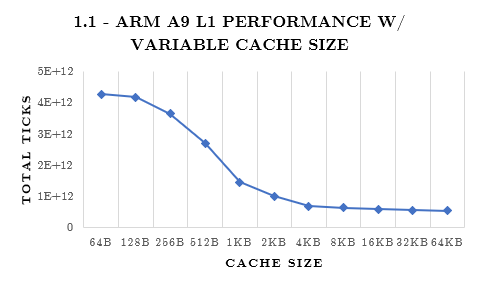
\includegraphics[scale=.5]{ex1_1.png}
\caption{Impact on number of ticks by varying the L1 cache size}
\label{figurelabel}
\end{figure}

\subsection{Associativity Level}

The next task is the set the L1 instruction and data cache sizes to a constant 2kB, while keeping the L2 cache disabled. Then the associativity is varied by the power, $n^2$, as non-squared powers deliver invalid results (and empty stat.txt files). 

\begin{table}[h]
\caption{ARM A9 - L1 Associativity and Total Ticks}
\label{table_example}
\begin{center}
\begin{tabular}{|c||c|}
\hline
Associativity & Total Ticks\\
\hline
1 & 1.00454E+12\\
\hline
2 & 7.27428E+11\\
\hline
4 & 6.87746E+11\\
\hline
8 & 6.83377E+11
\\
\hline
\end{tabular}
\end{center}
\end{table}


\begin{figure}[thpb]
\centering
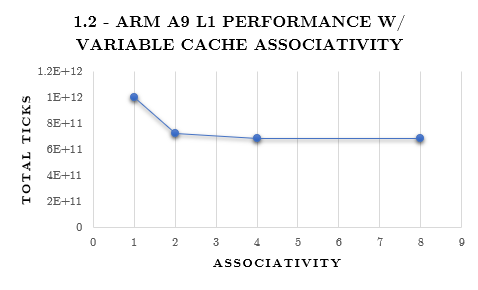
\includegraphics[scale=.5]{ex1_2.png}
\caption{Impact on number of ticks by varying the associativity level}
\label{figurelabel}
\end{figure}

\subsection{L2 Cache Size}

To explore the differences between varying the L1 and L2 cache sizes, the direct mapped L2 cache size is varied while the L1 cache sizes are now held constant. The performance is then analyzed with respect to the total processor ticks.


\begin{table}[h]
\caption{ARM A9 - L1 Associativity and Total Ticks}
\label{table_example}
\begin{center}
\begin{tabular}{|c||c|}
\hline
Cache Size & Total Ticks\\
\hline
2kB
 & 1.03179E+12
\\
\hline
4kB
 & 9.60558E+11
\\
\hline
8kB
 & 9.0899E+11
\\
\hline
16kB
 & 8.55049E+11
\\
\hline
\end{tabular}
\end{center}
\end{table}

\begin{figure}[thpb]
\centering
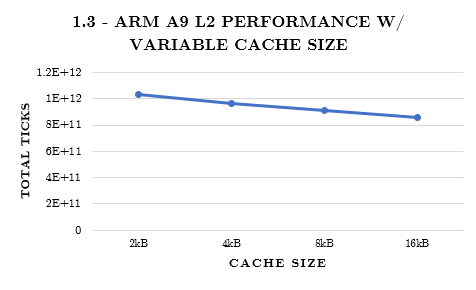
\includegraphics[scale=.5]{ex1_3.png}
\caption{Impact on number of ticks by varying the L2 cache size}
\label{figurelabel}
\end{figure}

\pagebreak

\section{ARM A15}

GEM5 can simulate very detailed models of processors. So far a model close to the ARM A9 core has been simulated. In the next simulation a model close to the ARM A15 core has been used.

The ARM A15 is simulated by using an out-of-order CPU that utilizes decoding, issuing, fetching and dispatching 3 instructions per cycle. It also incorporates two integer ALUs, one integer divider, one integer multiplier and a read/write port.

\begin{table}[h]
\caption{ARM A15 - L1 Cache Size and Total Ticks}
\label{table_example}
\begin{center}
\begin{tabular}{|c||c|}
\hline
Cache Size & Total Ticks\\
\hline
64B & 4.18925E+12
\\
\hline
128B & 4.13002E+12
\\
\hline
256B & 3.59686E+12
\\
\hline
512B & 2.62578E+12
\\
\hline
1kB & 1.36592E+12
\\
\hline
2kB & 8.97505E+11
\\
\hline
4kB & 5.56189E+11
\\
\hline
8kB & 4.9869E+11
\\
\hline
16kB & 4.49761E+11
\\
\hline
32kB & 3.95024E+11
\\
\hline
64kB & 3.87966E+11
\\
\hline

\end{tabular}
\end{center}
\end{table}

\begin{figure}[thpb]
\centering
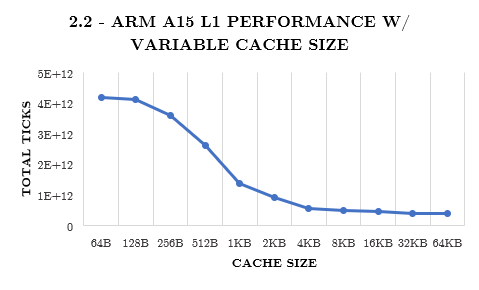
\includegraphics[scale=.5]{ex2_2.png}
\caption{Impact on number of ticks by varying the cache size}
\label{figure2_2}
\end{figure}

\section{Heterogeneous Platform A15-A15-A9-A9}
As a final experiment a heterogeneous multi-core platform consisting of two A15 cores and two A9 cores has been simulated. Each of the cores has a private L1 cache and the four cores use a shared L2 cache.

The test code for the eeg application has been modified to run on a multi-core platform using the OpenMP API. For-loops that have no dependencies between iterations have been preceded by a statement to run the iterations in parallel. This has been done for every for-loop in the application and the validity of the multi-core program has been tested by compiling it natively and by running a simulation on the heterogeneous platform.

The optimized values for the L1 cache have been chosen by finding the inflection point of the graphs in figures 1.1 and 2.2. For both the A15 and the A9 cores the optimal size of the cache is $1kB$. At the infliction point the trade-off between cost for larger cache and speed-up in number of cycles is optimal. The associativity is chosen as 2-way, because we see a large performance increase when the associativity is increased from 1 to 2, but the graph of figure 1.2 becomes very flat after that point.

For the L2 cache we can see in figure 1.3 that the larger this cache is, the faster the eeg application will run. $16kB$ is a feasible size for the L2 cache of the heterogeneous platform.

This platform performed 5.81 times faster on the eeg application than the single A9 core version and 1.27 times faster than the 3-core homogeneous A9 platform with comparable cache sizes.

%%%%%%%%%%%%%%%%%%%%%%%%%%%%%%%%%%%%%%%%%%%%%%%%%%%%%%%%%%%%%%%%%%%%%%%%%%%%%%%%
\newpage
\onecolumn
\section*{APPENDIX}

\begin{figure}[thpb]
\centering
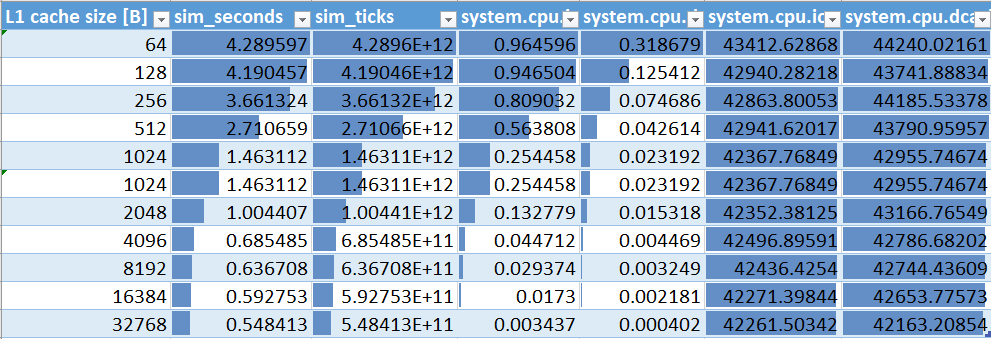
\includegraphics[scale=0.7]{Figures/assignment1_1_table.png}
\caption{A9: L1 cache size in bytes vs. sim\_seconds, sim\_ticks, L1 instruction cache miss rate, L1 data cache miss rate, L1 instruction cache average miss latency and L1 data cache average miss latency}
\label{Afigure1_1}
\end{figure}

\begin{figure}[thpb]
\centering
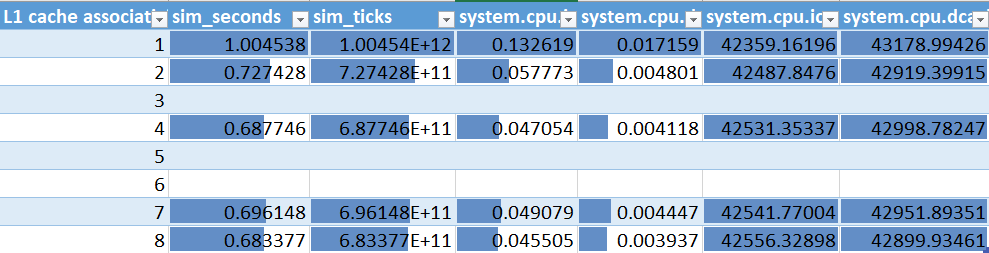
\includegraphics[scale=0.7]{Figures/assignment1_2_table.png}
\caption{A9: L1 cache associativity vs. sim\_seconds, sim\_ticks, L1 instruction cache miss rate, L1 data cache miss rate, L1 instruction cache average miss latency and L1 data cache average miss latency}
\label{Afigure1_2}
\end{figure}

\begin{figure}[thpb]
\centering
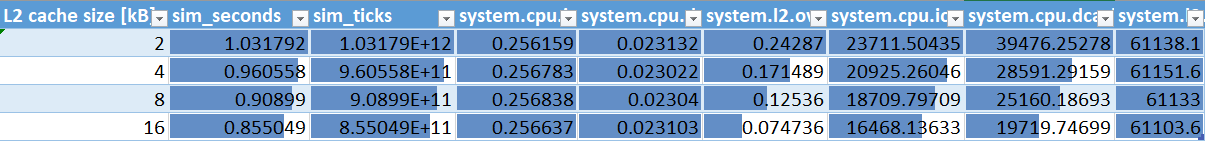
\includegraphics[scale=0.572]{Figures/assignment1_3_table.png}
\caption{A9: L2 cache size vs. sim\_seconds, sim\_ticks, L1 instruction cache miss rate, L1 data cache miss rate, L2 cache miss rate, L1 instruction cache overall average miss latency, L1 data cache overall average miss latency and L2 cache average miss latency}
\label{Afigure1_3}
\end{figure}

\begin{figure}[thpb]
\centering
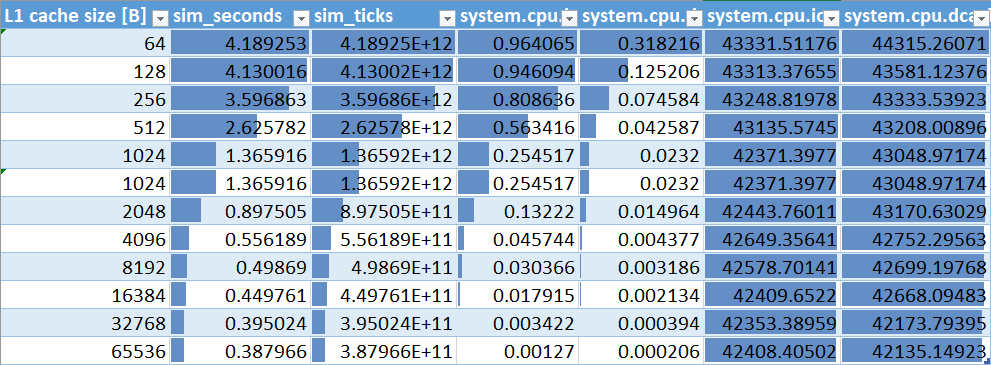
\includegraphics[scale=0.7]{Figures/assignment2_2_table.png}
\caption{A15: L1 cache size in bytes vs. sim\_seconds, sim\_ticks, L1 instruction cache miss rate, L1 data cache miss rate, L1 instruction cache average miss latency and L1 data cache average miss latency}
\label{Afigure2_2}
\end{figure}

\end{document}
